\section{Testing}

\subsection{Testing tools}

The Jmeter Testing tool was used during the testing part of the project. 

JMeter is a tool that helps measure the performance of applications that are using HTTP protocol. The Jmeter configuration consists of several test plans that each represent the set of actions made by clients. This approach gives necessary flexibility for this project. Several test plans that emulate requests to the main VMO were developed. For the current solution the tests plan consists of nine GET requests through HTTP protocol that return data model objects. On the other hand, for the solution with HVG, the test plan sends single POST request with JSON data that describes relations between DMOs. The Jmeter configuration is presented in Appendix B \ref{fig:jmeter_conf}. JMeter also builds the plot and the table of the request that was made with the corresponding time parameters.

\subsection{Performance Comparison of Redis and Web caches}

% describe jmeter configuration

During the project experiments, several configurations were conducted. The list of configurations is presented below:

\begin{itemize}
  \item Middleware server with Redis cache
  \item Middleware server with Varnish web cache
  \item Middleware server with Apache Traffic server cache
  \item Middleware server with HQL and second-level cache
  \item Middleware server with HQL, second-level cache and data compression
  \item Middleware server with HQL, second-level cache and first level cache
  \item Middleware server with HQL, second-level cache, first level cache and data compression
\end{itemize}

As can be seen, the tests are divided into two parts: configurations for testing internal cache replacement and configurations for testing VMO creation. The first part analyzes and evaluates performance of redis cache and web cache servers. The second part  evaluates HVG performance.
%  In the end the corresponding conclusion is made. 

Each experiment consists of several parts and can be described as an algorithm below: 

\begin{itemize}
  \item Configure Jmeter test plan
  \item Run Jmeter Test plan on predefined set of parallel request (which emulate users)
  \item Evaluate Summary Report
\end{itemize}

For each test, the next configuration was used: Jmeter emulates one hundred users that are making continuous requests for fetching the view model object of the main page.  


\subsection{Performance evaluation of Redis Cache and Web cache solutions}


\begin{figure}[h!]
    \centering
    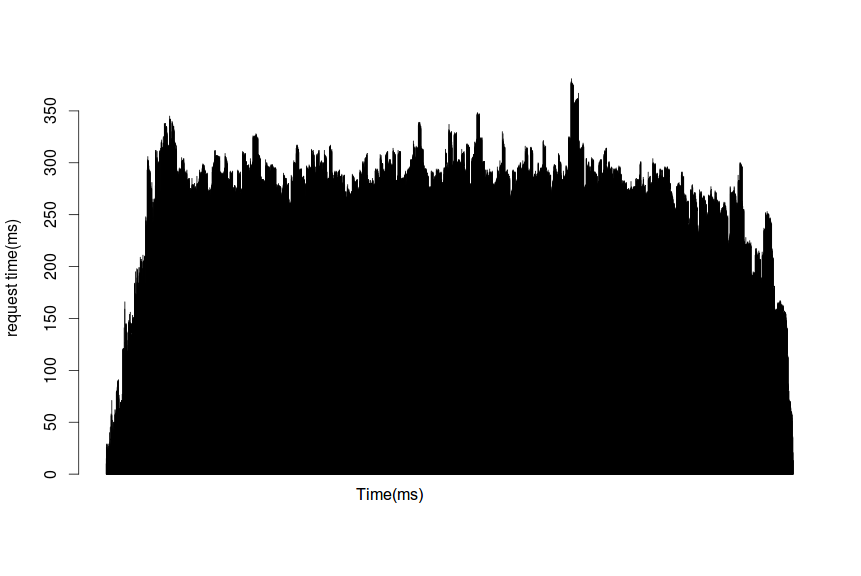
\includegraphics[width=15cm,height=7cm,keepaspectratio]{images/vmo_redis_mult_par.png}
    \caption{Response time of middleware server wihth Redis cache for generating VMO through parallel requests}
    \label{fig:vmo_redis_mult_par}
\end{figure}


\begin{figure}[h!]
    \centering
    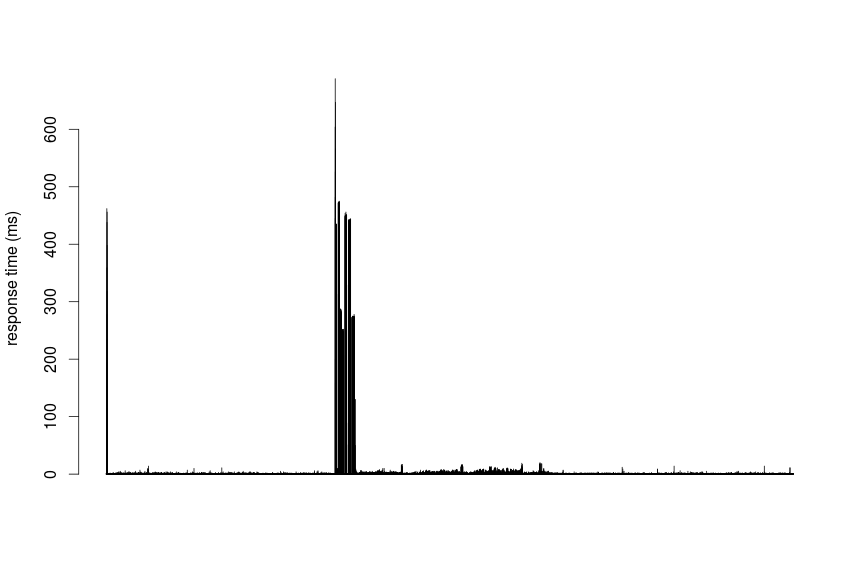
\includegraphics[width=15cm,height=7cm,keepaspectratio]{images/vmo_varnish_mult.png}
    \caption{Response time of Varnish web cache for generating hierarchical VMO}
    \label{fig:vmo_varnish_mult}
\end{figure}


This type of test emulates the user requests for generating view model object for the main page. In order to build a VMO, several requests should be done for gathering data model objects. The request for building a single page consists of nine REST subrequests through HTTP protocol for gathering DMOs. The corresponding Jmeter test plan is presented on figure \ref{fig:vmo_testplan}.

\begin{figure}[h!]
    \centering
    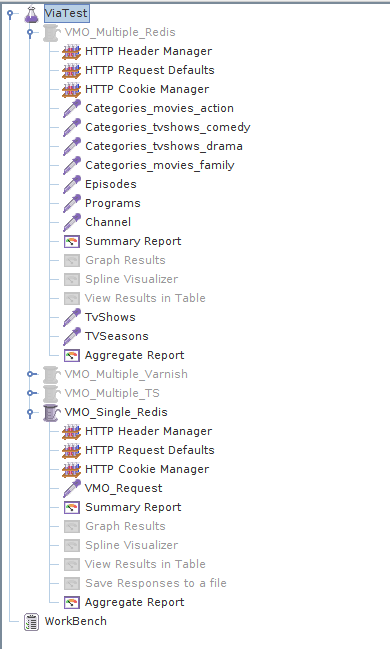
\includegraphics[width=10cm,height=10cm,keepaspectratio]{images/vmo_testplan.png}
    \caption{The Jmeter test plan for current solution and proposed solution with HVG}
    \label{fig:vmo_testplan}
\end{figure}

\begin{figure}[h!]
    \centering
    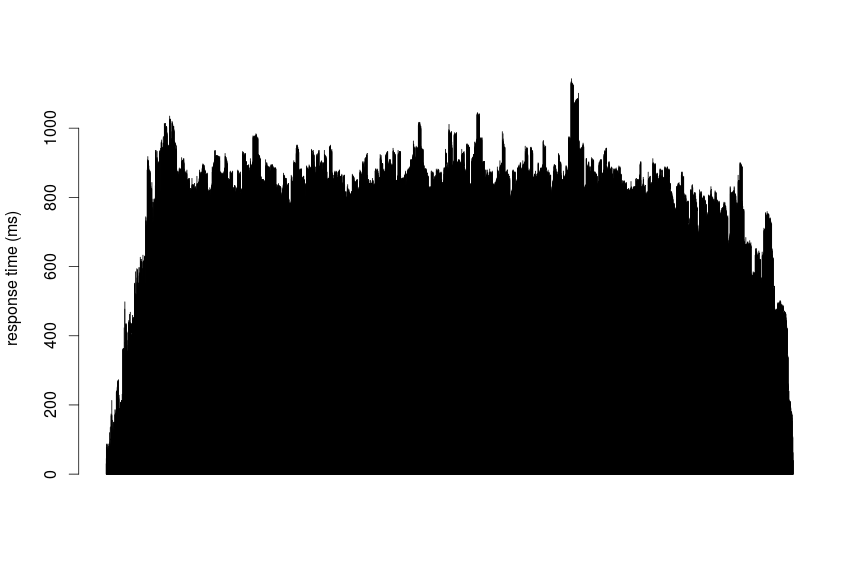
\includegraphics[width=15cm,height=7cm,keepaspectratio]{images/vmo_redis_mult_seq.png}
    \caption{Response time of middleware server with Redis cache for generating hierarchical VMO through sequential requests}
    \label{fig:vmo_redis_mult_seq}
\end{figure}

Figure \ref{fig:vmo_redis_mult_par} illustrates server response time for generating VMO that has no dependencies between objects. As can be seen, the maximum response time is about 300 ms. Figure \ref{fig:vmo_redis_mult_seq} shows response time from middleware server for generating hierarchical VMO that tree structure is shown on \ref{fig:vmo_test_example}. 

\begin{figure}[h!]
    \centering
    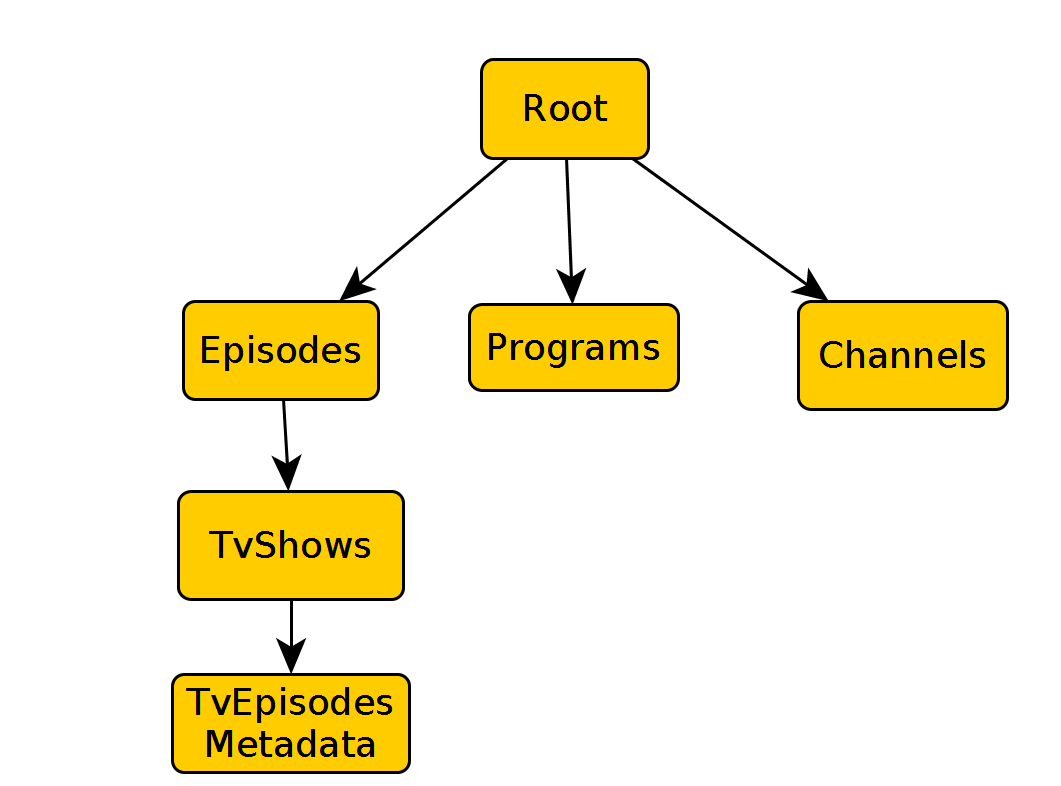
\includegraphics[width=15cm,height=7cm,keepaspectratio]{images/vmo_test_example.png}
    \caption{View Model Object that is used during testing}
    \label{fig:vmo_test_example}
\end{figure}


\begin{figure}[h!]
    \centering
    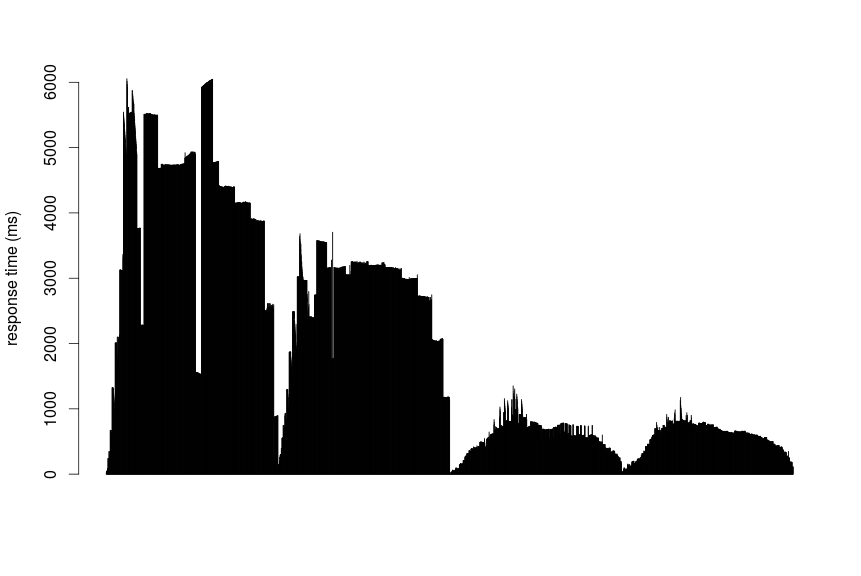
\includegraphics[width=15cm,height=7cm,keepaspectratio]{images/vmo_hvg.png}
    \caption{Response time of middleware server for generating hierarchical VMO through HVG}
    \label{fig:vmo_hvg}
\end{figure}


The VMO has tree structure with depth equal to three. The initial node is always called \textit{root}. It has no data and is introduced for convenience to "glue" other nodes in a tree. As can be noticed, it is the longest path (Root $\rightarrow$ Episodes $\rightarrow$ TvShows $\rightarrow$ TvEpisodesMetadata) and a has depth of four; As a result, three sequential requests should be made for generating data (the root node is excluded because it has no data). As shown, the performance decreases about three times. It is quite predictable because it is necessary to make three sequential requests. Figure \ref{fig:vmo_varnish_mult} shows the VMO generation through Varnish web cache. The response time decreases dramatically. The reason for this is that it takes constant time to get data from the Varnish web cache. The request for getting DMO rarely touches the middleware server. It is noticable from the figure, when the request goes through varnish web cache to the middleware server the response time increases. Figure \ref{fig:vmo_ts_mult} shows the response time for making requests through Apache Traffic server configured as a web cache. The results more predictable than the results of varnish web cache. The maximum time does not reach 100 ms.  

\begin{figure}[h!]
    \centering
    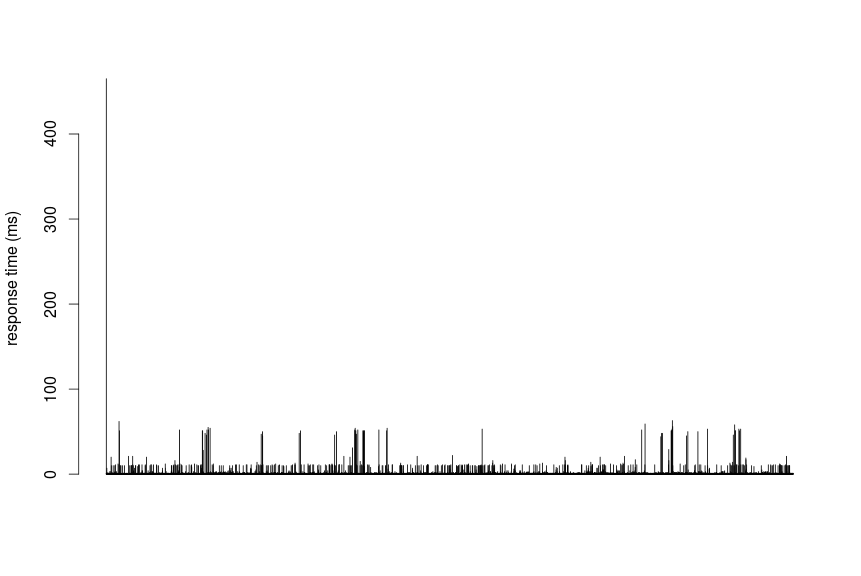
\includegraphics[width=15cm,height=7cm,keepaspectratio]{images/vmo_ts_mult.png}
    \caption{Response time of Apache Traffic Server for generating hierarchical VMO}
    \label{fig:vmo_ts_mult}
\end{figure}

\subsection{Performance evaluation of HVG with different configurations}

Figure \ref{fig:vmo_hvg} shows the response time for a hierarchical VMO generator with different configurations. As can be seen, there are four hills, each hill represents the corresponding experiment: HVG with first level cache (caching data model objects), HVG with first level cache and data compression, HVG with first and second level caches (caching both data model objects and view model objects) and HVG with first and second level cache and data compression. The first hill appears to be the slowest one, responses come in around 6000ms in the worst case. The behaviour is quite unpredictable, because the vmo requests consume 100\% of CPU and the amount of data that is transferred between client and middleware server is quite big.


The second hill is almost twice as fast as the first one. The reason for that being the  reduced amount of data transferred between client and server. The compression reduces the amount of data by almost five times. As can be seen, the compression does not produce overhead and slows responses for a negligible time. In addition, the hill looks more predictable and has less valleys.  


\begin{figure}[h!]
    \centering
    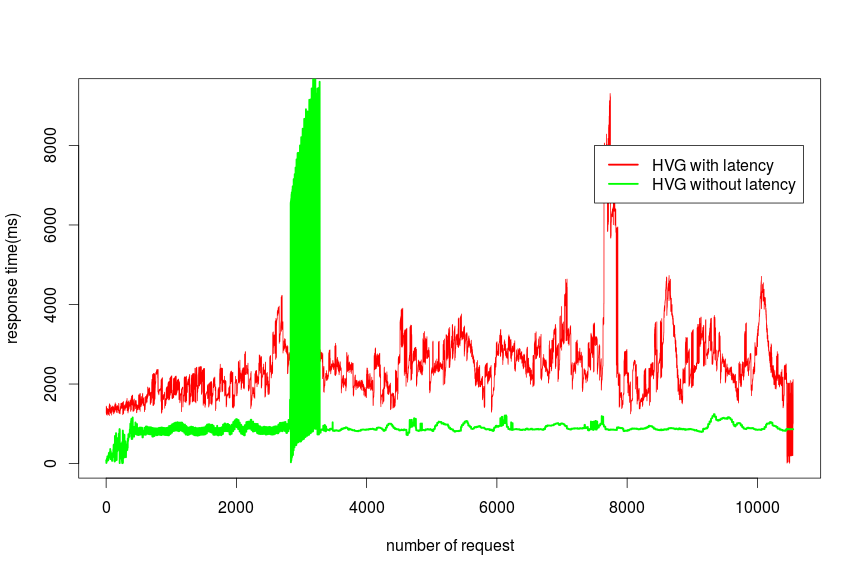
\includegraphics[width=15cm,height=7cm,keepaspectratio]{images/hvg_latency_comparison.png}
    \caption{Comparison of response time with and without latency for optimal HVG configuration}
    \label{fig:hvg_comparison}
\end{figure}


The third hill shows the response time from middleware server with two level caches. As can be seen, the server performs three times faster than hill number two and almost six times faster than the first hill. This happens because the middleware server rarely executes requests for building VMOs. It does checks if VMO is already computed every time before executing actual request. 

The last hill represents the response time with second and first level caches and data compression. It can be noticed that the hill is more stable than the third one, but the execution time is roughly the same.


\begin{figure}[h!]
    \centering
    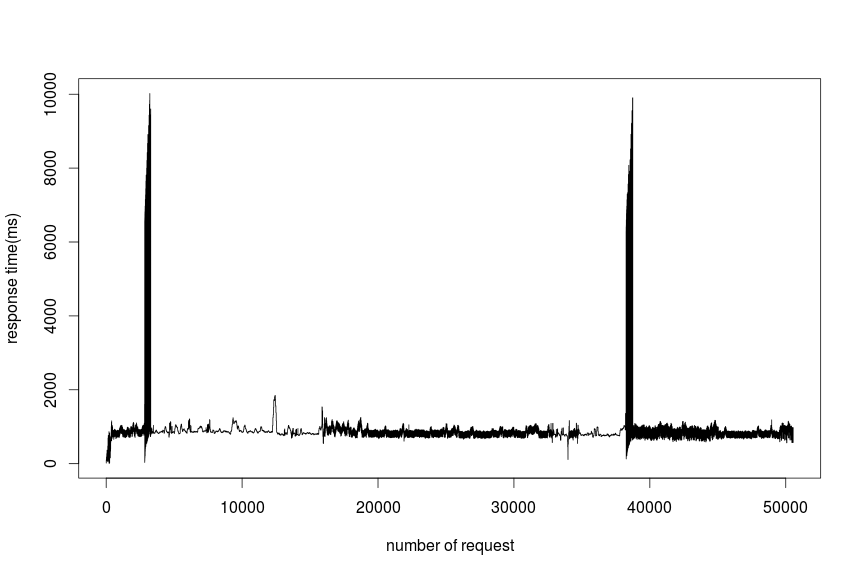
\includegraphics[width=15cm,height=7cm,keepaspectratio]{images/hql_loadtest.png}
    \caption{Load test of optimal HVG configuration}
    \label{fig:hvg_loadtest}
\end{figure}

The brief result is that the optimal configuration for HVG is two level cache and data compression.


Figure \ref{fig:hvg_loadtest} demonstrates the load test for optimal HVG configuration. During the test around 50000 (fifty thousand) requests were made in one hundred parallel threads. There are two peaks that can be observed that have response time around 10.000 msec. During these requests, the middleware server requested data from the underlying content distributor. There it can be seen that the mean response time is around ~1500 msec.


\begin{figure}[h!]
    \centering
    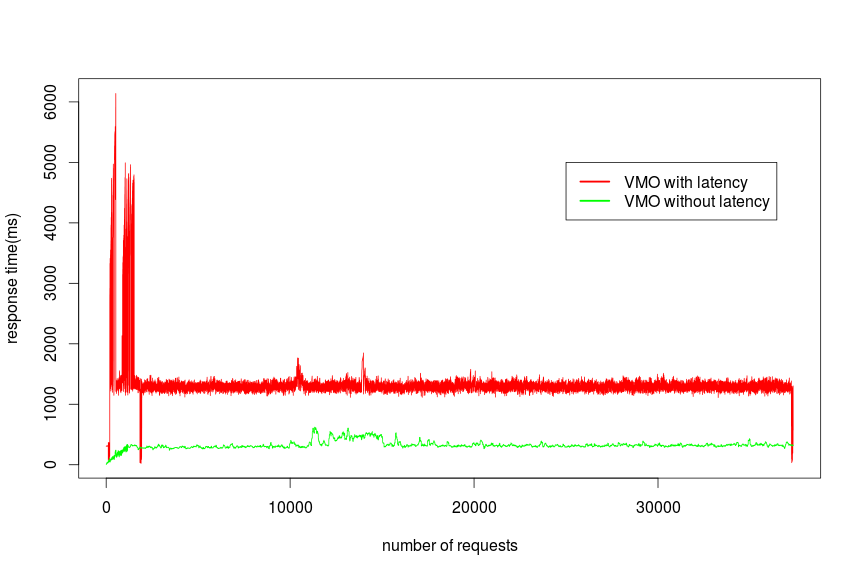
\includegraphics[width=15cm,height=7cm,keepaspectratio]{images/vmo_parallel_comparison.png}
    \caption{Comparison of response time with and without latency for VMO generation without dependencies using multiple requests}
    \label{fig:vmo_comparison}
\end{figure}

The tests executed up until this point were conducted without introducing latency. The next obvious step is to make an artificial latency and observe how the server response time depends on it. The artificial latency is about ~500 msec between client and server. Figure \ref{fig:hvg_comparison} shows the comparison between responses with artificial latency and without. As can be seen there is one big peak on the green plot, is appeared because several events happened at the same time: the data in the redis cache became stale and the redis server could not write data fast enough due to lack of resources. The red plot also has one peak, the reason for this is the stale data in redis cache and corresponding request to the content provider.

\begin{figure}[h!]
    \centering
    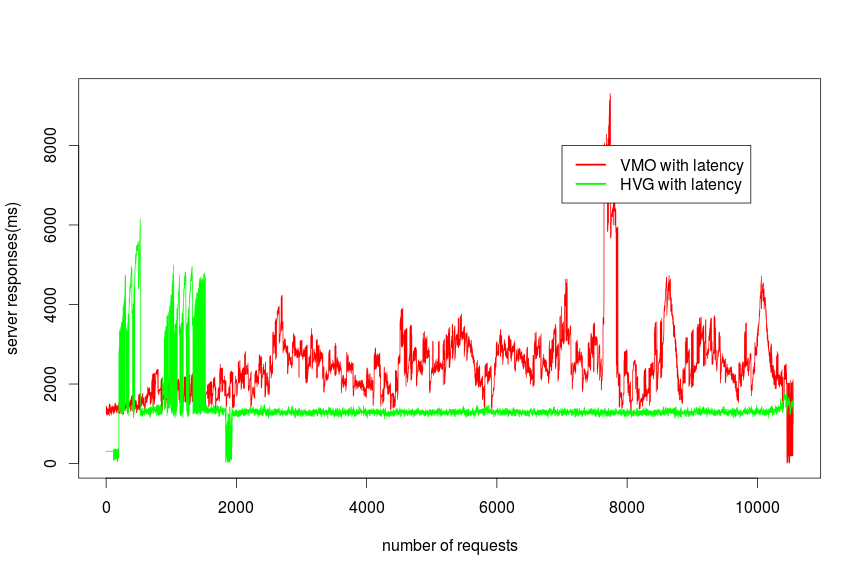
\includegraphics[width=15cm,height=7cm,keepaspectratio]{images/hvg_vmo_latency_comparison.png}
    \caption{Comparison of response time between parallel VMO generation and HVG with optimal configuration}
    \label{fig:hvg_vmo_latency_comp}
\end{figure}


The next figure \ref{fig:vmo_comparison} shows the comparison between responses with and without latency for generating VMO through multiple requests. There it can be observed that the server made several responses to the content distributor; As a result, the request time is about ~6000 msec. In some cases the response time for requests with latency is less than the response time without latency. It is a small persentage of errors during the experiments. When these errors occur, the server immediately sends an empty response.


Figure \ref{fig:hvg_vmo_latency_comp} shows the comparison between HVG with optimal configuration and VMO generated through multiple requests. As can be seen during the HVG test, several requests were made to the content distributor. The red plot also shows that the VMO through multiple requests also did several requests because of the stale content. Both plots had a small error during the experiment; as a result, server responses with approximately ~10 ms can be observed. The HVG with optimal configuration shows great performance compared to the VMO through multiple requests. In addition, it is more stable and reliable. 




\newpage

